\documentclass{exercise}
\usepackage{global-settings}
\usepackage{multicol}
\usepackage{subcaption}
\usepackage{booktabs} 
\usepackage{enumitem}
\usepackage[compat=1.1.0]{tikz-feynman}
\usepackage[version=4]{mhchem}

\def\modelsolution{1}

\setcounter{exercise}{1}
\release{Mittwoch, 04.12.2024}
\submission{Mittwoch, 11.12.2024, 14 Uhr}


\DeclareMathOperator\artanh{artanh}

\begin{document}

\clearpage
\makeheader

\exercise{Fragen (2P)}
Stellen Sie \emph{pro Person} zwei relevante Fragen zu den Inhalten der Vorlesung \enquote{Einf\"uhrung in die Kern- und Elementarteilchenphysik}.

\exercise{Quarksalat(2P)}

    In einem Kollisions-Experiment werden durch Protonkollisionen verschiedene Teilchen erzeugt. Dabei gilt besondere Aufmerksamkeit dem $\Lambda_c^+$ sowie dem $\overline{\Xi^{0}_{b}}$ in Verbindung mit anderen Teilchen, zusammengefasst als $X$, im Endzustand:
    %
    \begin{align*}
    %\pi^-+p & \rightarrow K^++X_1\\
    %p+p & \rightarrow \overline{\Lambda_c^+}+X
    p+p & \rightarrow \Lambda_c^+ + \overline{\Xi^{0}_{b}}+X
    \end{align*}
    %
    Betrachten Sie im Folgenden nur die starke Wechselwirkung.
    \begin{enumerate}
        \item Bestimmen Sie den Quarkinhalt des $\Lambda_c^+$ sowie des $\overline{\Xi^{0}_{b}}$.  
        \item Geben Sie die minimale Anzahl an Hadronen (Mesonen/Baryonen) an, aus denen $X$ bestehen muss. Nennen Sie explizite Teilchen für eine physikalisch korrekte Zusammensetzung des $X$. \\ (\emph{Hinweis}: Überlegen Sie auf Quarkniveau!)
        \item Die Energie des einen Protons im Laborsystem beträgt $\SI{7}{\giga\electronvolt}$. Leiten Sie allgemein her, wie groß die Energie des anderen Protons im Laborsystem mindestens sein muss, um alle Reaktionsprodukte aus (b) zu erzeugen. Ist dabei eine ultrarelativistische Näherung gerechtfertigt? Begründen Sie. Falls Sie (a) und (b) nicht bearbeitet haben, rechnen Sie mit zwei Teilchen der Massen $m_1 = \SI{8}{\giga\electronvolt}$ und $m_2 = \SI{8.6}{\giga\electronvolt}$ als Reaktionsprodukte.
    \end{enumerate}

    
    \solution{
    \begin{enumerate}
        \item $\Lambda_c^+$: Charmness $1$, Strangeness $0$, Beauty $0$.\\
            $\Rightarrow \overline{c}$ und 2 leichte Quarks; Ladung muss $+1$ sein $\rightarrow$ ($udc$). \\
            $\overline{\Xi^{0}_{b}}$: Charmness $0$, Strangeness $1$, Beauty $-1$ (da Antiteilchen).\\
                $\Rightarrow \overline{b} + \overline{s}$ und 1 leichtes Quark; Ladung muss $0$ sein $\rightarrow$ ($\overline{u}\overline{s}\overline{b}$).
            Nach der Kollision:
        %
        \begin{table}[htb]
        \centering
            \begin{tabular}{c
                                            c
                                            c
                                            c
                                            c
                                            c}
                \toprule
                {-} & {u} & {d} & {c} & {s} & {b} \\
                \midrule
                {Vor Kollision} & 4 & 2 & 0 & 0 & 0 \\
                {Nach Kollision} & 0 & 1 & 1 & -1 & -1 \\
                \bottomrule
            \end{tabular}
        \end{table}
        %
        \item Damit die Baryonenzahl erhalten ist, müssen noch mindestens zwei weitere Baryonen entstehen. Da aber rechts 8 Quarks ausgeglichen werden müssen, wird zusätzlich noch mindestens ein Meson benötigt $\rightarrow$ \textbf{mindestens 3 Teilchen}.
        Es müssen 4 up-Quarks, 1 down-Quark, 1 Anti-charm, 1 strange-Quark und ein beauty-Quark erzeugt werden. Dies ist möglich über $(\Lambda_b^0, D_s^-, \Delta^{++})$, $(\Xi_b^0, D^0, p)$, $(\Lambda_b^0, D^0,\Sigma^+)$, $(\Lambda^0, B_c^-, \Delta^{++})$ oder $(\Sigma^+, B_c^-,p)$, wie im Folgenden als Beispiel:	
        %
        \begin{table}[htb]
        \centering
            \begin{tabular}{l
                                            c
                                            c
                                            c
                                            c
                                            c}
                \toprule
                { } & {u} & {d} & {c} & {s} & {b} \\
                \midrule
                {Startbilanz} & -4 & -1 & 1 & 1 & -1 \\
                {Proton} & -2 & 0 & 1 & 1 & -1 \\
                {$B_{c}^-$} & -2 & 0 & 0 & 1 & 0 \\
                {$\Sigma^+$} & 0 & 0 & 0 & 0 & 0 \\
                \bottomrule
            \end{tabular}
        \end{table}
        %
        \item Aufstellen der 4er Impulserhaltung im Laborsystem:
        \begin{align*}
            &{p_{p1}^\mu} + {p_{p2}^\mu} = {p_{\Lambda_c^+}^\mu} + {p_{\overline{\Xi^{0}_{b}}}^\mu} + {p_{p}^\mu} + {p_{B_{c}^-}^\mu} + {p_{\Sigma^+}^\mu}\\
            &\begin{pmatrix}
             E_{p1}+E_{p2} \\
              \vec{p}_{p1}+\vec{p}_{p2} 
            \end{pmatrix} = 
            \begin{pmatrix}   
                {E_{\Lambda_c^+}} + E_{\overline{\Xi^{0}_{b}}} + {E_{p}} + {E_{B_{c}^-}} + {E_{\Sigma^+}}\\ \vec{p}_{\Lambda_c^+} + p_{\overline{\Xi^{0}_{b}}} + \vec{p}_{p}+\vec{p}_{B_{c}^-}+\vec{p}_{\Sigma^+} 
            \end{pmatrix} \\
            &{\begin{pmatrix}
             E_{p1}+E_{p2} \\
              \vec{p}_{p1}+\vec{p}_{p2} 
            \end{pmatrix}}^2 = 
            {\begin{pmatrix}   
                {E_{\Lambda_c^+}} + E_{\overline{\Xi^{0}_{b}}} +  {E_{p}} + {E_{B_{c}^-}} + {E_{\Sigma^+}}\\ 
                0
            \end{pmatrix}}^2
        \end{align*}
        Da man an der Erzeugungsschwelle interessiert ist, wird im letzten Schritt das Bezugssystem auf der rechten Seite so gewählt, dass die Impulse der Tochterteilchen jeweils Null sind. Damit ist $E_i = m_i$ und für die Energie der Protonenstrahlen ergibt sich:
        \begin{align*}
        &2m_p^2 + 2E_1E_2-2\vec{p}_1\vec{p}_2 = (m_{\Lambda_c^+} + m_{\overline{\Xi^{0}_{b}}} + m_{p} + m_{B_{c}^-} + m_{\Sigma^+})^2\\
        &4E_1E_2 = - 2m_p^2 + (m_{\Lambda_c^+} + m_{\overline{\Xi^{0}_{b}}} + m_{p} + m_{B_{c}^-} + m_{\Sigma^+})^2\\
        &E_1 = \frac{(m_{\Lambda_c^+} + m_{\overline{\Xi^{0}_{b}}} + m_{p} + m_{B_{c}^-} + m_{\Sigma^+})^2 - 2m_p^2}{4E_2}
        \end{align*}
        Das Quadrieren der Viererimpulse ist hier essentiell, da die Strahlenergien asymmetrisch sind und das gesuchte Laborsystem nicht dem Ruhesystem der Produkte entspricht. Es wird also auf den Seiten der Gleichung in verschiedenen Bezugssystemen gerechnet.\\
        
        Die Massen der Teilchen:
        %
        \begin{align*}
            &m(\Lambda_c^+ + \overline{\Xi^{0}_{b}}) = (2286 + 5949)\,\si{\mega\electronvolt}= \SI{8235}{\mega\electronvolt}  \\
            &m_1(\Sigma^+ + B_{c}^- + p) = (1189 + 6275 + 938)\,\si{\mega\electronvolt} = \SI{8402}{\mega\electronvolt} \\
            &m_2(\Delta^{++} + D_s^- + \Lambda_b^0) = (1230 + 1968 + 5624)\,\si{\mega\electronvolt} = \SI{8822}{\mega\electronvolt} \\
            &m_3(\Xi_b^0 + D^0 + p) = (5949 + 1865 + 938)\,\si{\mega\electronvolt} = \SI{8752}{\mega\electronvolt} \\
            &m_4(\Lambda_b^0 + D^0 + \Sigma^+) = (5624 + 1865 + 1189)\,\si{\mega\electronvolt} = \SI{8678}{\mega\electronvolt} \\
            &m_5(\Lambda^0 + B_{c}^- + \Delta^{++}) = (1116 + 6275 + 1230)\,\si{\mega\electronvolt} = \SI{8621}{\mega\electronvolt} 
        \end{align*}
        Das Ergebnis lautet: $E_1 = \SI{9826}{\mega\electronvolt}$. \\
        Der $\beta$-Faktor beträgt dann $0.99$ für eine Protonenergie von $7\,$GeV. Demzufolge ist eine ultrarelativistische Näherung gerechtfertigt. 
    
        \end{enumerate}
        Punkte (Vorschlag):
        \begin{enumerate}
        \item Quarkinhalt (2P)
        \item Anzahl Teilchen und Teilchenkandidaten (5P)\\
        \item Energieberechnung (2.5P) + Rechtfertigung Näherung (0.5P)
    \end{enumerate}
    }


\section{Schwache Wechselwirkung (10P)}

In dieser Aufgabe untersuchen Sie den Zerfall eines Myon $\mu^- \to e^- \overline{\nu}_{e} \nu_\mu$. 
Da die Bestimmung Berechnung der Übergangswahrscheinlichkeit nicht Teil dieser Vorlesung ist, beschränkt sich diese Aufgabe auf den Beginn und das Ende der notwendigen Berechnung.

\begin{enumerate}
    \item Erklären Sie kurz, was die V-A Struktur der schwachen Wechselwirkung beschreibt und was dies für die Teilchen bedeutet, die schwach wechselwirken.
    \solution{Vektor - Axialvektor bedeutet, dass die schwache WW nur an linkshändigen Teilchen koppelt. Mathematisch ist $\left( 1 - \gamma^5 \right)$ der linkshändige Projektor, welcher dazu führt, dass Parität maximal gebrochen wird.}


    \item Der Übergang $\Gamma_{i \to f}$ von einem Anfangszustand $\mu^- $ zu einem Endzustand $e^- \overline{\nu}_{e} \nu_\mu $ kann durch Fermis Goldene Regel beschrieben werden.
    Geben Sie diese an und beschreiben Sie ihre Komponenten.
    \solution{
        $\Gamma_{i \to f} = \dfrac{2\pi}{\hbar} \left| M_{f,i}\right|^2 \mathrm{d} \Pi_\text{LIPS}$ Das Matrixelement $M_{f,i}$ beschreibt die Amplitude des Übergangs, und $\mathrm{d} \Pi_\text{LIPS}$ beschreibt die Anzahl der möglichen Endzustände.
    }





    \item Zeichnen Sie das Feynman-Diagramm, welches den Zerfall des $\mu^-$ auf Tree-Level beschreibt.
    \solution{
    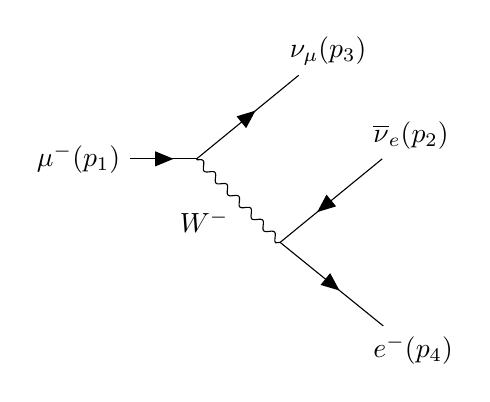
\begin{tikzpicture}
        \begin{feynman}
          \vertex (a) {\(\mu^{-}(p_1)\)};
          \vertex [right=of a] (b);
          \vertex [above right=of b] (f1) {\(\nu_{\mu}(p_3)\)};
          \vertex [below right=of b] (c);
          \vertex [above right=of c] (f2) {\(\overline \nu_{e}(p_2)\)};
          \vertex [below right=of c] (f3) {\(e^{-}(p_4)\)};
      
          \diagram* {
            (a) -- [fermion] (b) -- [fermion] (f1),
            (b) -- [boson, edge label'=\(W^{-}\)] (c),
            (c) -- [anti fermion] (f2),
            (c) -- [fermion] (f3),
          };
        \end{feynman}
      \end{tikzpicture}
    }

\end{enumerate}
Der nächste Schritt ist es das Matrixelement über die Feynman-Regeln zu bestimmen und den Phasenraum über Integrale der Vierervektoren zu bestimmen.
Diese Rechung wurde Ihnen bereits abgenommen, sodass nur ein letztes Integral verbleit. 
Die Zerfallsrate in Abhängigkeit der Elektronenenergie $E_\text{e}$ ist gegeben durch 
\begin{equation}
    \dfrac{\mathrm{d} \Gamma}{\mathrm{d} E_\text{e}} = \left(\dfrac{g_\text{w}}{M_\text{W}c}\right)^4 \dfrac{m_\mu^2 E^2_\text{e}}{2\hbar \left( 4 \pi\right)^3} \cdot \left(1 - \dfrac{4 E_e}{3 m_\mu c^2}\right) \,.
\end{equation}
Zunächst müssen die Integrationsgrenzen bestimmt werden. Vernachlässigen Sie die Ruhemassen der Produkte.
\begin{enumerate}[resume] 
    \item Bestimmen Sie die obere Integrationsgrenze von $E_\text{e}$. 
    \item Argumentieren Sie, dass für die untere Grenze, dass das Elektron in Ruhe $E_\text{e} = 0$ erzeugt werden kann.  

    \item Führen Sie nun die Integration aus und geben Sie eine Gleichung für die Lebenszeit eines $\mu^-$ an.
    \solution{
        \begin{align}
            \Gamma =& \left(\dfrac{g_\text{w}}{M_\text{W}c}\right)^4 \dfrac{m_\mu^2}{2\hbar \left( 4 \pi\right)^3}
            \int_{0}^{1/2 m_\mu c^2} E^2\left( 1 - \dfrac{4E}{3m_\mu c^2}\right) \, \mathrm{d}E \\
                =& \left(\dfrac{m_\mu g_\text{w}}{M_\text{W}}\right)^4 \dfrac{m_\mu c^2}{12 \hbar \left(8 \pi \right)^3}
        \end{align}
        Für die Lebenszeit gilt $\tau = \dfrac{1}{\Gamma}$\,.
    }

    \item Vergleichen Sie das Ergebnis mit dem Literaturwert. Erklären Sie mögliche Abweichungen.
    \solution{
        Es entstehen Abweichungen, weil hier nur Tree-Level Diagramme betrachtet werden.
        Es werden die Ruehmassen vernachlässigt.
    }
\end{enumerate}
    
\end{document}